\documentclass[xcolor=x11names,compress,professionalfonts]{beamer}

%% General packages %%%%%%%%%%%%%%%%%%%%%%%%%%%%%%%%%%
\usepackage[utf8]{inputenc}
\usepackage{graphicx}
\usepackage{tikz}
\tikzset{% change default arrow tips
    >=latex
}
\usepackage{ifthen}

\usepackage{amsmath}
\usepackage{nicefrac}

\usepackage{color}

%%%%%%%%%%%%%%%%%%%%%%%%%%%%%%%%%%%%%%%%%%%%%%%%%%%%%%


%% Beamer Layout %%%%%%%%%%%%%%%%%%%%%%%%%%%%%%%%%%
\useoutertheme[subsection=false,shadow]{miniframes}
\useinnertheme{rectangles}

\setbeamertemplate{navigation symbols}{}%remove navigation symbols

\newcommand{\btVFill}{\vskip0pt plus 1filll}%place an element at the bottom of the page

\usepackage{libertine}
\usepackage[T1]{fontenc}

\setbeamerfont{title like}{shape=\scshape}
\setbeamerfont{frametitle}{shape=\scshape}

\setbeamercolor*{lower separation line head}{bg=DeepSkyBlue4} 
\setbeamercolor*{normal text}{fg=black,bg=white} 
\setbeamercolor*{alerted text}{fg=red} 
\setbeamercolor*{example text}{fg=black} 
\setbeamercolor*{structure}{fg=black} 
 
\setbeamercolor*{palette tertiary}{fg=black,bg=black!10} 
\setbeamercolor*{palette quaternary}{fg=black,bg=black!10} 

\renewcommand{\(}{\begin{columns}}
\renewcommand{\)}{\end{columns}}
\newcommand{\<}[1]{\begin{column}{#1}}
\renewcommand{\>}{\end{column}}

\newcommand{\om}{\ensuremath{\tau^{-1}}}
\newcommand{\lb}{\ensuremath{\overline{\lambda}}}
\newcommand{\zb}{\ensuremath{\overline{z}}}
\newcommand{\ham}{\ensuremath{H}}

\definecolor{BostonBlue}{HTML}{00688B}
\definecolor{Complementary}{HTML}{8B2300}
%%%%%%%%%%%%%%%%%%%%%%%%%%%%%%%%%%%%%%%%%%%%%%%%%%

\usepackage{braket}
% compile child documents using this preamble
\usepackage{subfiles}

%%%My Math

\newcommand{\pd}[2]{\frac{\displaystyle \partial #1}{\displaystyle\partial #2}} % for partial derivatives
\newcommand{\dx}{\mathrm{d}x}
\renewcommand{\d}[1]{\mathrm{d}#1}
\newcommand{\nth}{$n^\text{th}$ }

\newcommand{\mean}[1]{\langle #1 \rangle}
\DeclareMathOperator{\Pf}{Pf}
\DeclareMathOperator{\Tr}{Tr}

\begin{document}


\begin{frame}
\title{Multifractality of the tight-binding eigenstates on the Fibonacci chain}
%\subtitle{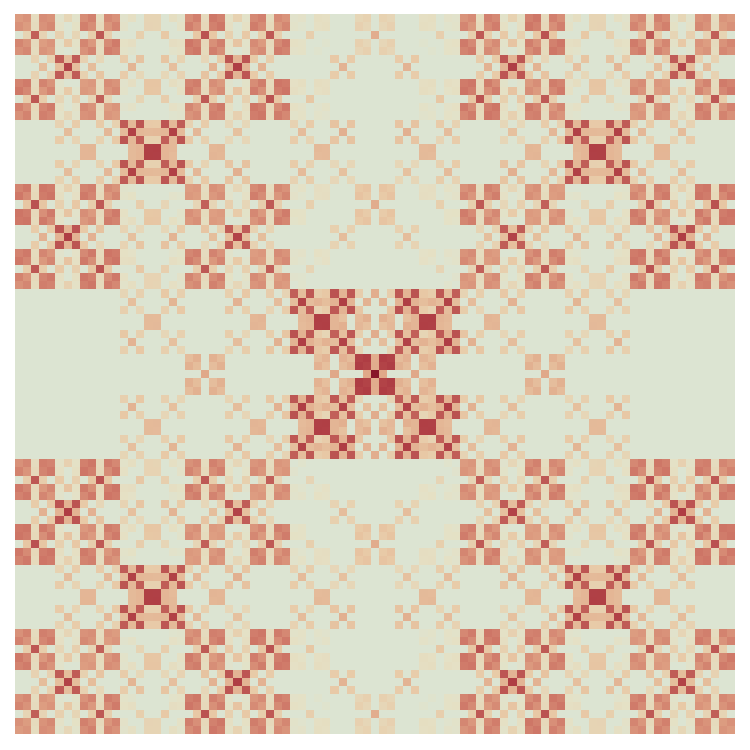
\includegraphics[width=0.2\textwidth]{illustration.pdf}}

%\titlegraphic{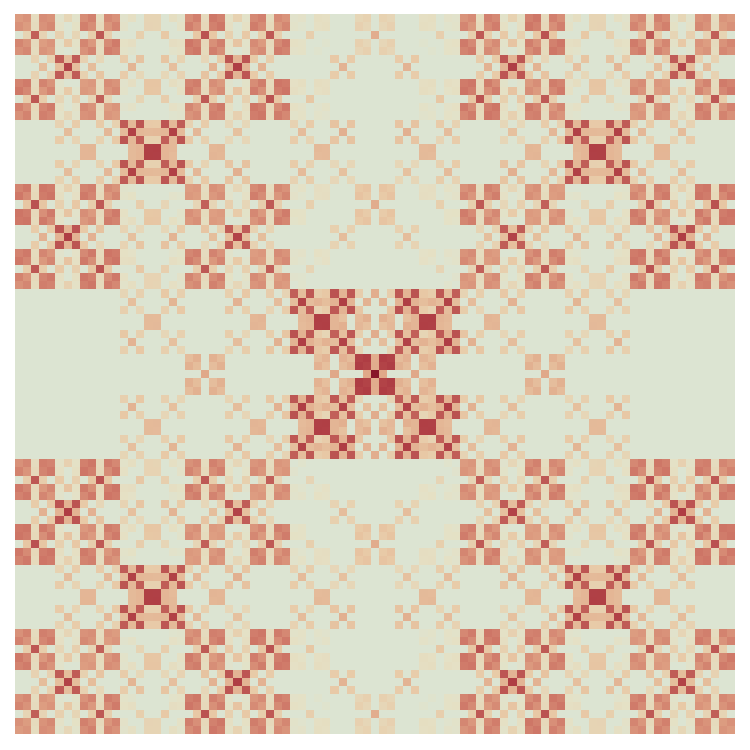
\includegraphics[width=0.4\textwidth]{illustration.pdf}}

\author{ Nicolas Macé, Anuradha Jagannathan, Frédéric Piéchon}

\institute % (optional)
{
  Laboratoire de Physique des Solides\\
  Université Paris-Sud
}

\date{November 25, 2015}

\titlepage

\btVFill
\begin{columns}
\begin{column}{2cm}
~\\
~\\
~\\
~\\
\raggedright

\includegraphics[scale=.15]{LogoUPSUD.png}
\end{column}
\begin{column}{6cm}
\centering
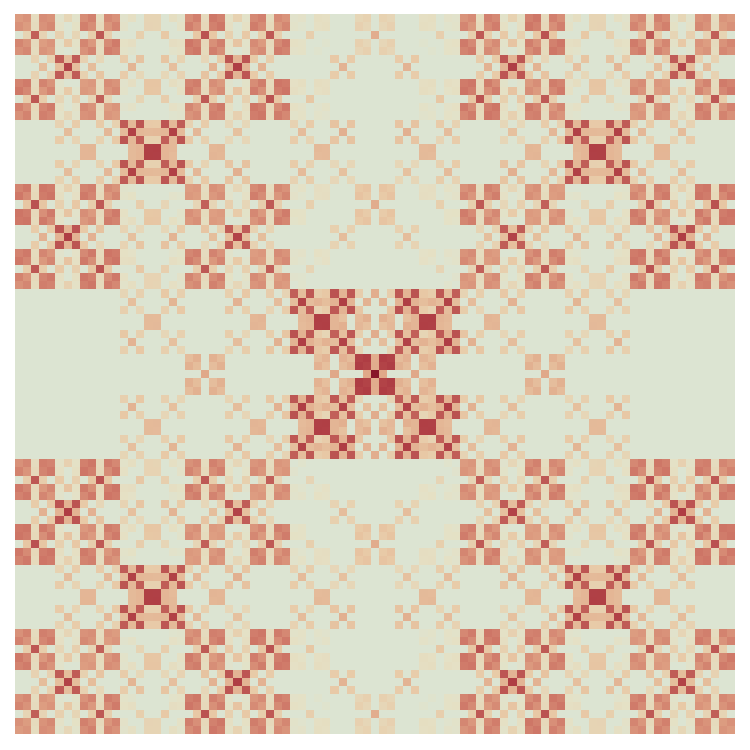
\includegraphics[width=.5\textwidth]{illustration.pdf}
\end{column}
\begin{column}{2cm}
~\\
~\\
~\\
~\\
\raggedleft

\includegraphics[scale=.15]{logo-lps.jpg}
\end{column}
\end{columns}
\end{frame}

\begin{frame}
\frametitle{Outline}
\tableofcontents[hideallsubsections]
\end{frame}

\section{The pure hopping Fibonacci Hamiltonian.}
%Each section needs a subsection for the small points on top to show up
\subsection{Dummy}

\begin{frame}{The pure hopping Fibonacci Hamiltonian}
\begin{columns}
\begin{column}{8.5cm}
	\centering
	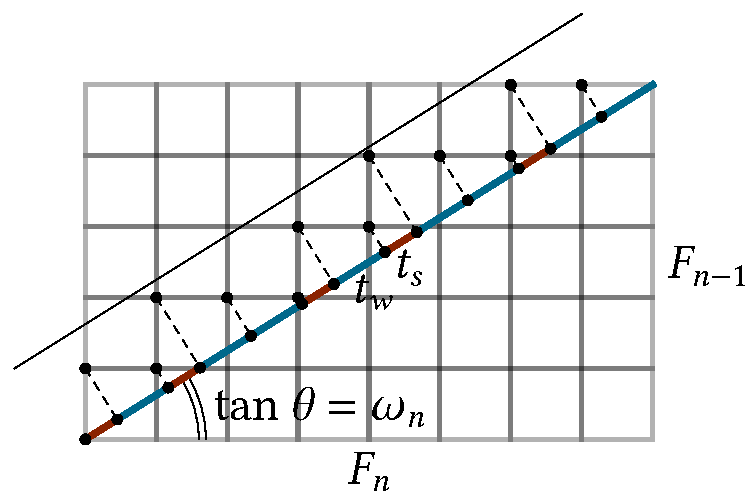
\includegraphics[scale=.7]{cut_and_project.pdf}
\end{column}

\begin{column}{3cm}
\begin{align*}
\omega_n &= \frac{F_{n-1}}{F_{n}} \\
\omega_n &\rightarrow \tau^{-1} = \frac{\sqrt{5}-1}{2}
\end{align*}
\begin{align*}
\rho &= \frac{t_w}{t_s} < 1 \\
\rho &\rightarrow 1 \scriptsize{\text{ (weak modulation)}} \\
\rho &\ll 1 \scriptsize{\text{ (strong modulation)}}
\end{align*}
\end{column}
\end{columns}

	Hamiltonian of the n$^\text{th}$ approximant:
	\[ \ham_n = - \sum_i t_i^{(n)} \ket{i} \bra{i+1} + \text{h.c.} \]
\end{frame}

\begin{frame}{Perturbative renormalization group on the Fibonacci chain}
	\centering
	\begin{itemize}
	\item Atomic RG step (decimation of molecules) \subfile{atomic_deflation.tex}
	\item Molecular RG step (decimation of atoms) \subfile{molecular_deflation.tex}
	\end{itemize}
	\begin{flushright}
	$z= \rho/2$, $\zb = \rho^2$ (Niu \& Nori 1986, Kalugin, Kitaev \& Levitov 1986)
	\end{flushright}
\end{frame}

\begin{frame}{RG reconstruction of the energy spectrum}
 \[ H_n = \underbrace{\left( z H_{n-2} - t_s \right)}_{\text{bonding levels}} + \underbrace{\left( \zb H_{n-3} \right)}_{\text{atomic levels}} + \underbrace{\left( z H_{n-2} + t_s \right)}_{\text{antibonding levels}} + \mathcal{O}(\rho^4)\]
	$\rightarrow$ simple recursive construction of the spectrum (Piéchon \emph{et al} 1995)
	
	\begin{columns}
	\begin{column}{6cm}
	\centering
	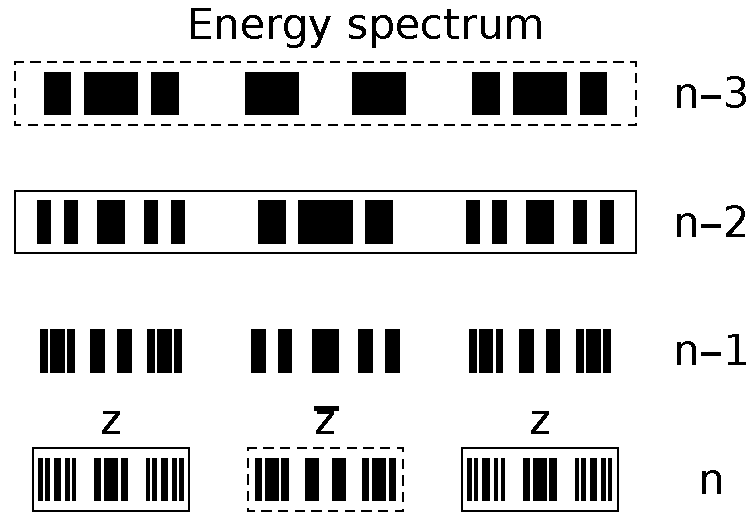
\includegraphics[scale=.4]{recursive_construction_spectrum.pdf}
	\end{column}
	\begin{column}{6cm}
	%\subfile{energy_tree.tex}
	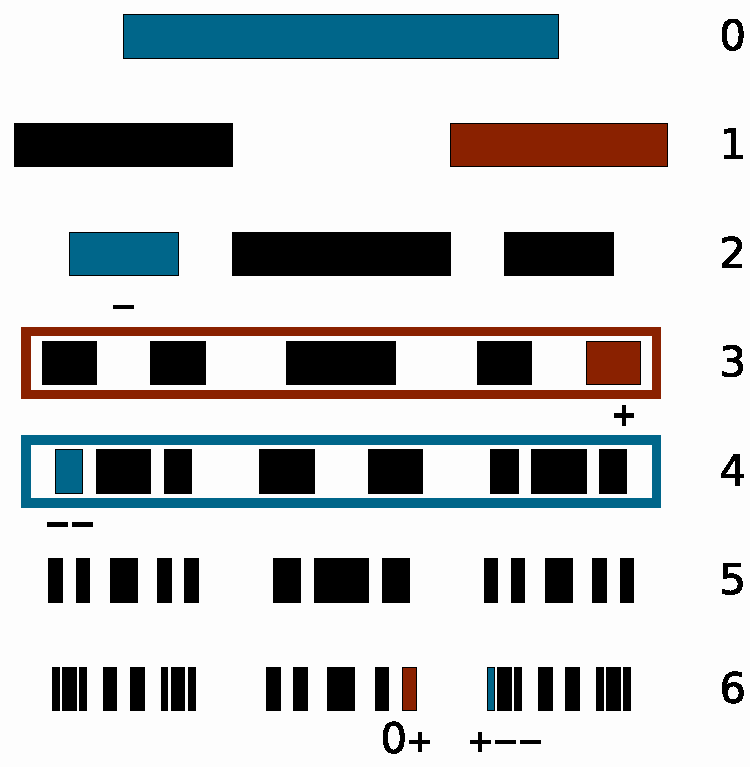
\includegraphics[scale=.3]{renormalization_paths_spectrum.pdf}
	%Renormalization paths characterized by
	%\[ x(E) = \frac{n_+ + n_-}{n} \]
	%\[
	%	x(\text{\scriptsize{central band}}) = 0, x(\text{\scriptsize{edge bands}}) = 1/2
	%\]
	\end{column}
	\end{columns}
	Renormalization paths characterized by
	\[ 
		x(E) = \frac{n_+ + n_-}{n} 
	\]
	\[ 
		x(\text{\scriptsize{central band}}) = 0, x(\text{\scriptsize{edge bands}}) = 1/2
	\]
\end{frame}

\section{The energy spectrum and its multifractal properties.}
\subsection{Dummy}

\begin{frame}{Multifractal analysis of the spectrum}

	\begin{itemize}
		\item Scale-invariant spectrum/idos
		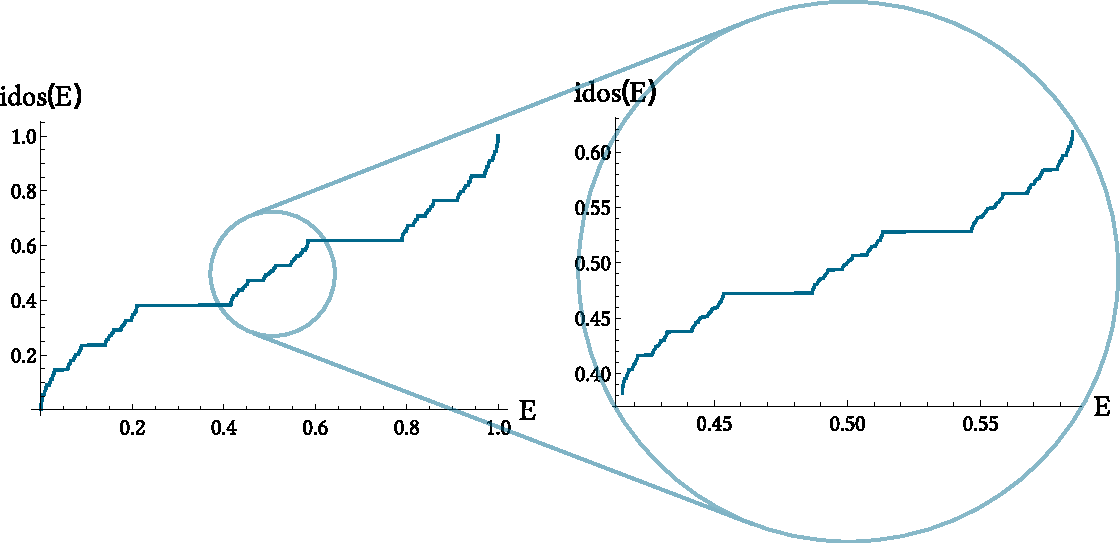
\includegraphics[scale=.4]{idos.pdf}
		
		\item $\implies$ locally, the idos is a scaling law of exponent $\alpha$
	
		\begin{align*}
		\alpha(x) &= \log \tau^{-1}/\left( x \log z/\zb^{2/3} + \log \zb^{1/3} \right) \\
		f(x) &= \frac{x \log \left(\frac{3 x}{2}\right)- (x+1) \log (x+1)^{1/3}+ (1-2 x) \log (1-2 x)^{1/3}}{\log \tau^{-1}}
	\end{align*}
	\begin{flushright}
	(Piéchon \emph{et al} 1995, Rüdinger \& Piéchon 1998)
	\end{flushright}
	\end{itemize}
\end{frame}

\section{The wavefunctions and their multifractal properties.}
\subsection{Dummy}
\begin{frame}{Fractal dimensions of the wavefunctions}
	\centering
	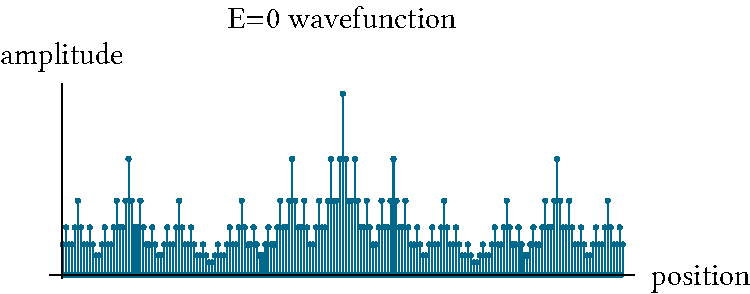
\includegraphics[scale=.55]{E0_wavefunction.pdf}
	\[
	\text{Scaling properties of $\psi$:~} 
	\sum_i |\psi_i^{(n)}(E)|^{2q} \sim (1/F_n)^{(q-1)D_q^\psi(E)} 
	\]
	\begin{align*}
	D_q(E) = 0/1 &\implies \text{extended/localized state}  \\
	0 < D_q(E) < 1 &\implies \text{critial state}
	\end{align*}
\begin{itemize}
	\item Wavefunctions at $E=0$ are critical (Kohmoto)
%	\item Averaged fractal dimensions of the wavefunction known to lowest order  (Thiem \& Schreiber 2013)
	\item Our work: use the RG approach to determine individual wavefunctions, and compute their fractal dimensions
\end{itemize}
\end{frame}

\begin{frame}{Perturbative RG for the wavefunctions}
%We relate the wavefunctions of $H_n$ to the wavefunctions of $H_{n-2}$, $H_{n-3}$:
	\begin{itemize}

		\item Atomic RG
			\begin{columns}
			\begin{column}{9cm}
				\subfile{rg_atomic_wavefunctions_main_txt.tex}
			\end{column}
			\begin{column}{2cm}
			\[ \lb \sim \frac{1}{1+2\rho^2}
			\]
			\end{column}
			\end{columns}
		\item Molecular RG
			\begin{columns}
			\begin{column}{9cm}
				\subfile{rg_molecular_wavefunctions_main_txt.tex}
			\end{column}
			\begin{column}{2cm}
			\[ \lambda \sim \frac{1}{2+\rho^2}
			\]
			\end{column}
			\end{columns}
	\end{itemize}

\[
	\begin{cases}
		|\psi_i^{(n)}(E)|^2 = \lb |\psi_{i'}^{(n-3)}(E')|^2 \text{~if $E$ is in the central cluster}\\
		|\psi_i^{(n)}(E)|^2 = \lambda |\psi_{i'}^{(n-2)}(E')|^2 \text{~if }E\text{~is in the edge clusters}
	\end{cases}
	\]
\end{frame}

\begin{frame}{Renormalization paths and fractal dimensions of the wavefunctions}
\begin{itemize}
	\item Fractal dimensions of the wavefunction of energy $E$:
	\[ \sum_i |\psi_i^{(n)}(E)|^{2q} \sim (1/F_n)^{(q-1)D_q^\psi(E)}  \]
	\item RG step neglecting sites with small amplitudes:
		\begin{align*}
			\text{molecular RG step:~} &|\psi_i^{(n)}(E)|^{2q} = \lambda^q |\psi_{i'}^{(n-2)}(E')|^{2q} \\
			\text{atomic RG step:~} &|\psi_i^{(n)}(E)|^{2q} = \lb^q |\psi_{i'}^{(n-3)}(E')|^{2q}
		\end{align*}
	\item $D_q^\psi(E)$ depends on the renormalization path $x(E)$:
	\[ (q-1)D_q^\psi(x) = \log \Bigg[ \left( \frac{\lambda(\rho)^q}{\lambda(\rho^q)} \right)^x \left( \frac{\bar{\lambda}(\rho)^q}{\bar{\lambda}(\rho^q)} \right)^{(1-2x)/2} \Bigg]/\log \omega \]
\end{itemize}
\end{frame}

\begin{frame}{Comparison with exact diagonalisation}
\begin{columns}
	\begin{column}{5cm}
		\centering
  		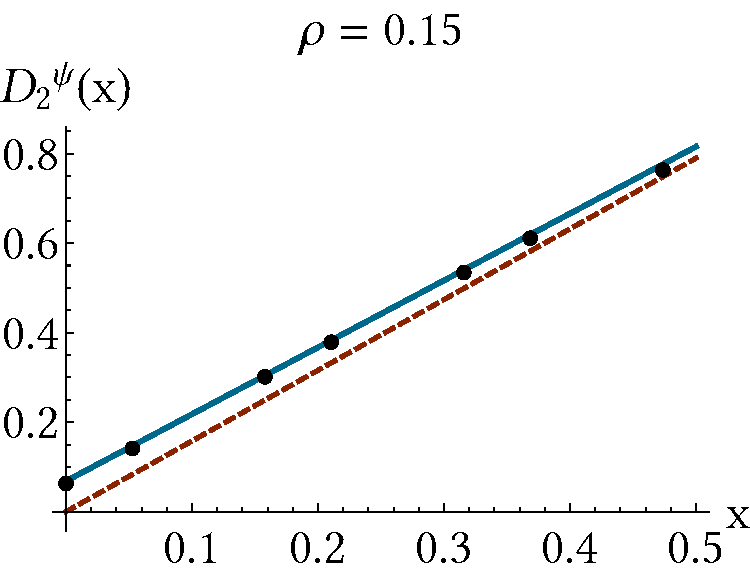
\includegraphics[scale=.4]{local_wf.pdf}
  		
  		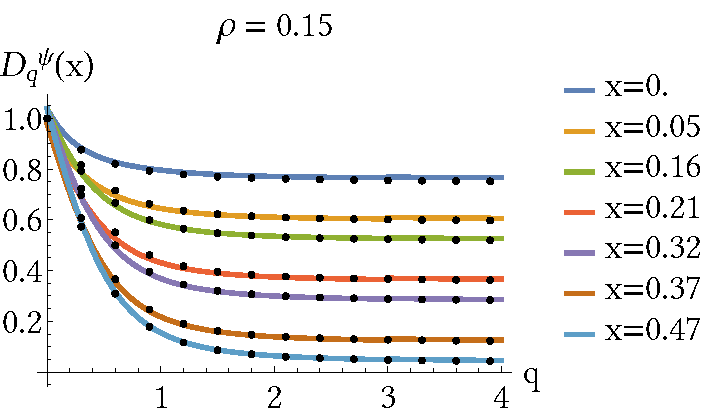
\includegraphics[scale=.48]{individual_wf_dimensions.pdf}
	\end{column}
	\begin{column}{6cm}
		%\begin{itemize}
		%	\item Multifractal behaviour well described
		%	\item All states are critical in the strong modulation limit
		%	\item Their multifractal character is captured by our description
		%	\item $x$ is the relevant parameter to describe the properties of the states
		%\end{itemize}
		
		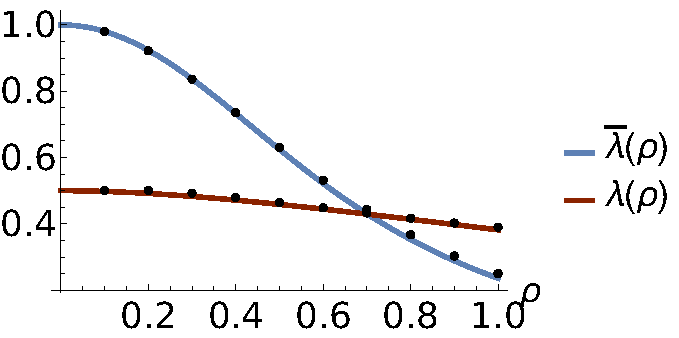
\includegraphics[scale=.5]{renorm_th_num.pdf}
		
		\begin{itemize}
			\item All states are critical in the strong modulation limit
			\item $x$ is the relevant parameter to describe the properties of the states
		\end{itemize}
		
		\begin{flushright}
		\scriptsize{(Macé, Jagannathan, Piéchon, in preparation)}
		\end{flushright}
	\end{column}
\end{columns}
\end{frame}

\begin{frame}{Energy averaged multifractality of the wavefunctions}
\[ 
	\frac{1}{F_n} \sum_E \sum_i |\psi_i^{(n)}(E)|^{2q}  \sim (1/F_n)^{(q-1)\bar{D}_q^\psi}
\]

{
\centering

		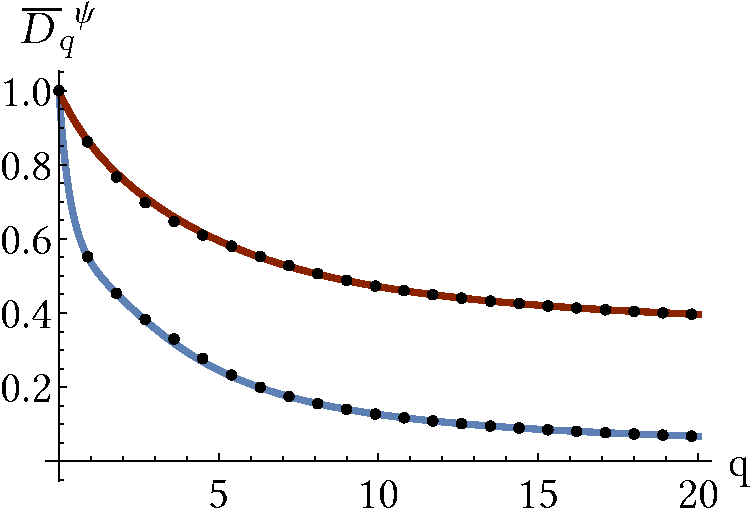
\includegraphics[scale=.55]{dq_av.pdf}		
		
}

%\begin{columns}
%	\begin{column}{5cm}
%		\centering
%		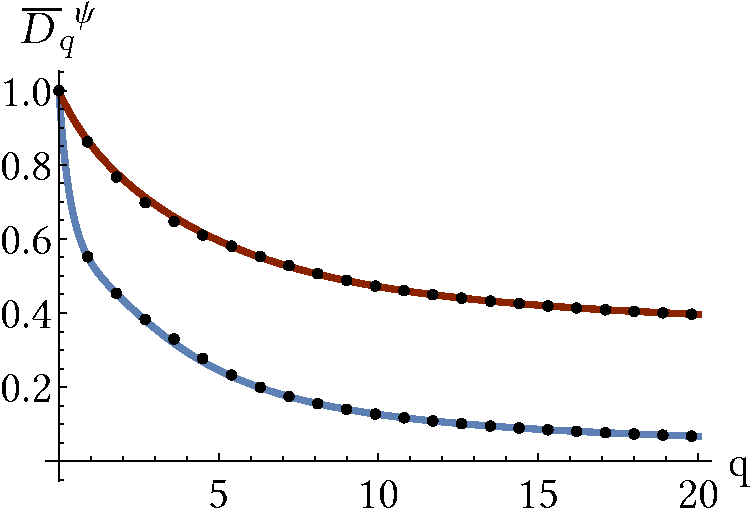
\includegraphics[scale=.4]{dq_av.pdf}
%	\end{column}
%	\begin{column}{5cm}
%		\centering
%		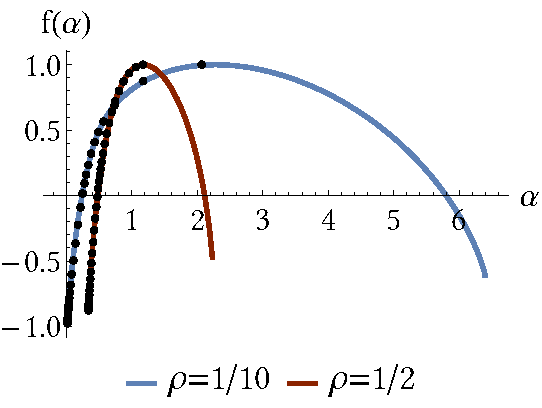
\includegraphics[scale=.6]{falpha_av.pdf}
%	\end{column}
%\end{columns}
		\begin{itemize}
			\item Multifractality
			\item Quantitative agreement with numerical data even for large $\rho$.
		\end{itemize}

\end{frame}

\begin{frame}{Seeing the fractality in superspace}
		{\centering
		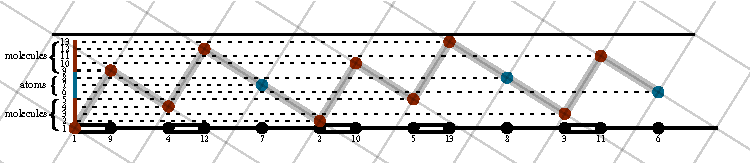
\includegraphics[scale=.85]{inclined_cut_and_project.pdf}
		
		}
		
		\begin{flushright}
		(Mosseri 1988)
		\end{flushright}
		
		\begin{columns}
	\begin{column}{7cm}
		\centering
		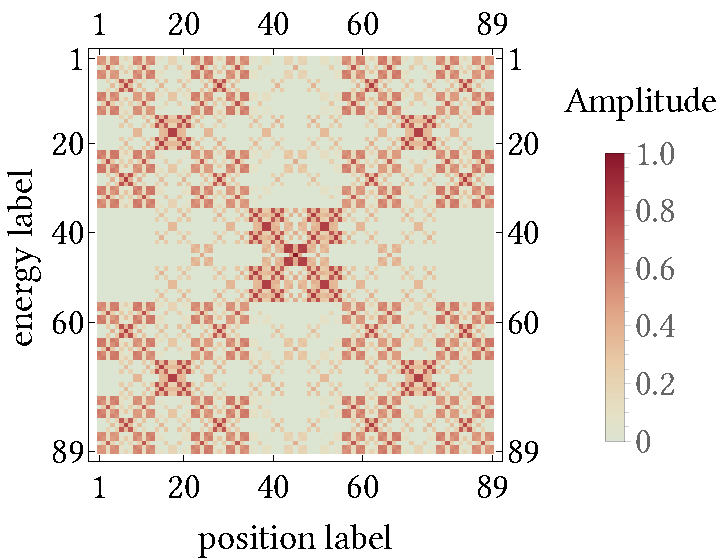
\includegraphics[scale=.4]{ldos_reordered.pdf}
		
		\scriptsize{Amplitude of the wavefunctions}	
	\end{column}
	\begin{column}{6cm}
		\begin{itemize}
			\item In perpendicular space, the fractal structure is obvious.
			\item Energy/position symmetry appears clearly.
		\end{itemize}
	\end{column}
\end{columns}
		
\end{frame}

\section{Conclusion}
\subsection{Dummy}
\begin{frame}{Conclusion and perspectives}
\begin{itemize}
	\item Fractal dimensions are important for physical properties such as transport and susceptibility.
	\item We have characterized the wavefunctions of the Fibonacci tight-binding chain, in the strong modulation limit, using a perturbative RG.
	\item We have presented for the first time analytical expressions for the fractal exponents of the full set of wavefunctions. These compare well with numerical data.
	\item Superspace description is meaningful for the physical properties of a quasicrystal.
	\item Work in progress: consequences for the diffusion and transport properties.
\end{itemize}
\end{frame}

\begin{frame}{Special thanks to...}
\begin{itemize}
	\item Anu Jagannathan, my supervisor,
	\item Frédéric Piéchon, our collaborator. \\
			$\rightarrow$ If you want to learn more about our work, go see his conf at geo-dyn2015, november 30 in Paris!
\end{itemize}

\centering

	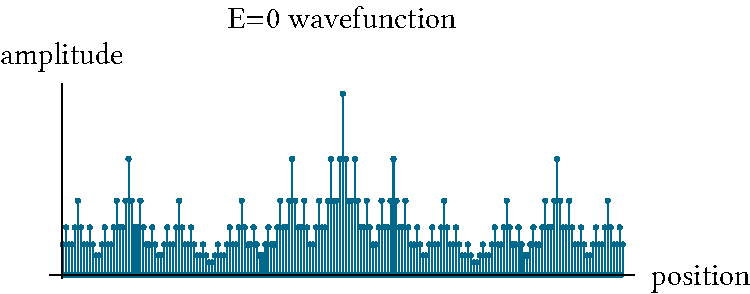
\includegraphics[scale=.55]{E0_wavefunction.pdf}	
	
\huge{Thank \emph{you} for your attention! \\Questions?}

\end{frame}

\begin{frame}
Nonperturbative expression for the renormalization factors:
\begin{align*}
\label{eq:lb}
	\lb(\rho) &= \frac{\sqrt{(1+\rho^2)^4+4\rho^4}-(1+\rho^2)^2}{2\rho^4}\\
	\lambda(\rho) &= \frac{1+\rho^2 \gamma(\rho) - \sqrt{1+(\rho^2 \gamma(\rho))^2}}{2 \rho^2\gamma(\rho)} \\
	\gamma(\rho) &= \frac{1}{1+\rho}
\end{align*}
\end{frame}

\end{document}
